\documentclass[12pt]{fithesis2}

% ===== LOADING PACKAGES =====
% language settings, main documnet language last
\usepackage[english]{babel}
% enabling new fonts support (nicer)
\usepackage{lmodern}
% setting input encoding
\usepackage[utf8]{inputenc}
% setting output encoding
\usepackage[T1]{fontenc}
% fithesis2 requires csquotes
\usepackage{csquotes}

\usepackage{subfig}
\usepackage{graphicx}
\usepackage{kpfonts}
\usepackage[labelfont=bf]{caption}
\usepackage{stmaryrd}
\usepackage{mathtools}
\usepackage[usenames, dvipsnames]{color}
\usepackage{esvect}
\usepackage{url}
\usepackage{dsfont}

\newcounter{counter}[section]
\renewcommand{\thecounter}{\thesection.\arabic{counter}}
\newenvironment{definition}[1]{\bigskip\refstepcounter{counter}\noindent\textbf{Definition \thecounter } \textit{#1} \par\nopagebreak}{\bigskip}
\newenvironment{example}[1]{\bigskip\refstepcounter{counter}\noindent\textbf{Example \thecounter} \textit{#1} \par\nopagebreak}{\bigskip}
\newenvironment{notation}{\bigskip\refstepcounter{counter}\noindent\textbf{Notation \thecounter}\par\nopagebreak}{\bigskip}
\newenvironment{proof}{\bigskip\refstepcounter{counter}\noindent\textbf{Proof \thecounter}\par\nopagebreak}{\bigskip}
\newenvironment{runningExample}[1]{\bigskip\refstepcounter{counter}\noindent\textbf{Running example \thecounter} \textit{#1} \par\nopagebreak}{\bigskip}

\newcommand\mdoubleplus{\mathbin{+\mkern-7mu+}}

\usepackage[
    backend=biber,      % use biber as backend instead of BiBTeX
    style=alphabetic,   % citation style
  url=true,           % display urls in bibliography
  hyperref=auto,      % detect hyperref and create links
    firstinits=true,    % abbreviate first names to initials
    maxbibnames=5,      % maxiumim number of authors before making 'et al.'
    alldates=iso8601,   % set date format to ISO 8601
]{biblatex}
\addbibresource{thesis.bib}
% setting custom colors for l

% FI THESIS settings
\thesistitle{Formal biochemical space for specification and analysis of biochemical processes}
\thesissubtitle{Master thesis}
\thesisstudent{Matej Troják}
\thesiswoman{false}
\thesisfaculty{fi}
\thesisyear{autumn 2017}
\thesisadvisor{RNDr.\ David Šafránek,\ Ph.D.}
\thesislang{en}

% ===== BEGIN DOCUMENT =====
\begin{document}

\FrontMatter
\ThesisTitlePage

\begin{ThesisDeclaration}
\DeclarationText
\AdvisorName
\end{ThesisDeclaration}

\begin{ThesisThanks}
Many thanks to you all.

\vspace{1em}
\noindent
There would be much less
algebra,        % advancements, art, adrenaline, archery, astrophotography, algebra
board gaming,   % beauty, baking, beer, board gaming
curiosity,      % courage, contemplation, cooking, cakes, curiosity
drama,          % discipline, devotion, drama
experience,     % empathy, experience
functional programmig,  % fun, friendliness, faith, functional programmig
geekiness,      % GEB, good books, geekiness
honesty,        % humour, honesty
inspiration,    % improvements, ideas, idealisms, inspiration
joy,            % jokes, joy
knowledge,      % knowledge
learning,       % learning, love
magic,          % meaning, magic, miracles, meta, moose
nighttime walks,    % nighttime walks, Norway
OpenLabs,       % organization, openness, optimism, OpenLabs
puzzle hunts,   % peace, patience, procrastination, puzzle hunts
quiet,          % quiet
respect,        % research, respect
surprises,      % spontaneity, silence, security, stories, star gazing, surprises
trust,          % typographic correctness, tolerance, trust
unpredictability,   % understanding, unity, unpredictability
vigilance,      % vigilance
Wachumba,       % wisdom, Wachumba
xylophone,      % xylophone
yummies         % yellow, you, yummies
and
zeal            % Zendo, Zen, zeal
in the world for me without you.

\vspace{0.65\textheight}
\noindent
Access to computing and storage facilities owned by parties and projects contributing to the National Grid Infrastructure MetaCentrum, provided under the programme Projects of Large Infrastructure for Research, Development, and Innovations(LM2010005), is greatly appreciated.
\end{ThesisThanks}

\begin{ThesisAbstract}
This thesis explores the randomness of outputs created by authenticated encryption schemes submitted to the  competition. Tested scenarios included three different modes of public message numbers. For the assessment, four different software tools were used: three common statistical batteries and a novel genetically inspired framework. The obtained results are interpreted in two ways: Firstly, to gain insights into the quality of the proposed  candidates. Secondly, to compare and contrast the used randomness testing tools. Directions for future research are proposed based on the obtained conclusions.
\end{ThesisAbstract}

\begin{ThesisKeyWords}
statistical randomness, authenticated encryption, CAESAR, evolutionary algorithms, genetic programming
\end{ThesisKeyWords}

\MainMatter
\tableofcontents

\chapter{Introduction}

\chapter{Background}

In our last paper~\cite{Ded201627}, we defined semantics of Biochemical Space Language (BCSL) via translating to a similar language called Kappa~\cite{Kappa}. However, we realised this approach is not very beneficial since we are not fully using the expressive power of our language this way. The thing is Kappa operates purely on expressions. We want to promote our language to a higher level when it operates on objects in multisets. By translating to Kappa we loose such abstraction. 

\section{Rule-based basics}
\label{Rule-based basics}

bla bla some intro

The reason for this kind of abstraction is the way how we see the biological models. We represent model $\mathcal{M}$ as set of rules and an initial solution of interacting entities. We understand solution as a mixture of individual objects which are randomly distributed (see Fig.~\ref{solutions:fig}a). Therefore, we cannot assign them any order and we do not see them as expressions but rather as multisets. For us, this representation of solution is the closest to the reality.

\begin{figure}
\begin{center}
\subfloat[]{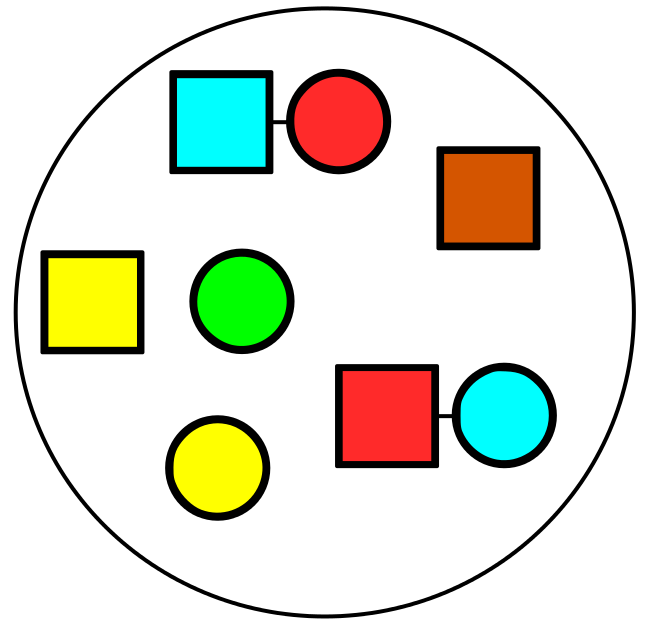
\includegraphics[scale=0.23]{pics/solution_first}\label{sol:s1}}
\hspace*{1cm}
\subfloat[]{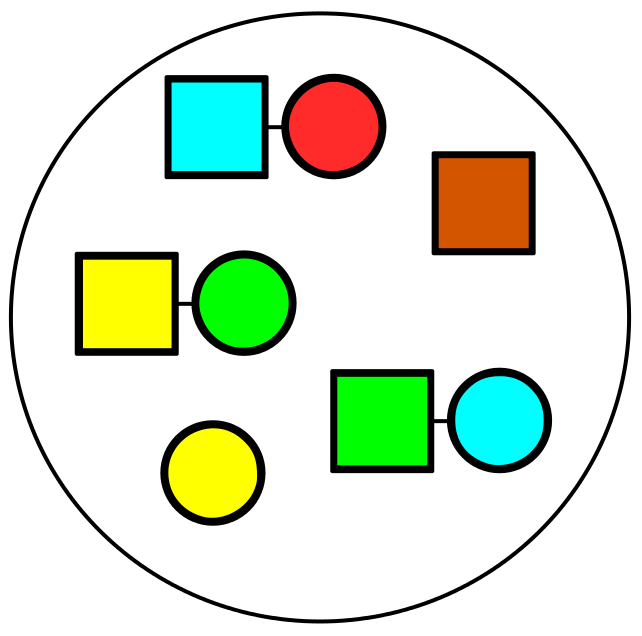
\includegraphics[scale=0.23]{pics/solution_second}\label{sol:s2}}
\caption{\textbf{Examples of solutions}. \textbf{(a)} An example of graphical representation of a solution. \textbf{(b)} Updated solution after rules from Fig.~\ref{rules:fig} were applied. The first rule \textit{(a)} was applied on the yellow $\square$ and green $\bigcirc$ and produced yellow-green complex $\square$--$\bigcirc$. Note there are more options how the rule could be mapped -- each combination of free $\square$ and $\bigcirc$. The second rule \textit{(b)} was applied on red-cyan complex $\square$--$\bigcirc$ where the color of $\square$ was changed from red to green. The third rule \textit{(c)} couldn't be applied because there is no such complex with yellow $\bigcirc$. }
\label{solutions:fig}
\end{center}
\end{figure}

On the other hand, the rules are expressions which describe behavior of groups of objects. A rule has form of a chemical reaction, where substrates and products take place. The difference is that reaction only operates on particular objects. Therefore, a reaction can be seen as a special case of rule (see Fig.~\ref{rules:fig}), where the groups contain exactly one element.

The rule can be mapped on a solution. Then, if it is mapped, it can be applied and a new solution is produced. The mapping is not always successful (see Fig.~\ref{solutions:fig}, application of rule \textit{c}). By repeating map-apply action, we obtain a \textit{Labelled transition system} $\mathcal{L}$.

\begin{def}\label{lts}
\textit{Labelled transition system} (LTS) $\mathcal{L}$ is a tuple $(S, A, \Delta, s_0)$ where:
\begin{itemize}
  \item $S$ is a (potentially infinite) set of states (solutions)
  \item $A$ is a set of labels (reactions)
  \item $\Delta \subseteq S \times A \times S$ is a transition relation (the map-apply action)
  \item $s_0 \in S$ is the initial state (initial solution)
\end{itemize}
\end{def}

\begin{figure}[!h]
\begin{center}
\begin{minipage}[l]{0.1\textwidth}
    \textbf{(a)}
  \end{minipage}
  \begin{minipage}[r]{0.6\textwidth}
    {\hspace*{0.8cm}
\includegraphics[scale=0.2]{pics/rule_complex}}
\end{minipage}

\begin{minipage}[l]{0.1\textwidth}
    \textbf{(b)}
  \end{minipage}
  \begin{minipage}[r]{0.6\textwidth}
    {\hspace*{1.35cm}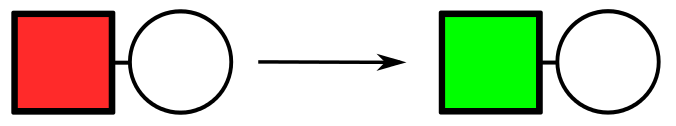
\includegraphics[scale=0.2]{pics/rule_change}}
\end{minipage}

\begin{minipage}[l]{0.1\textwidth}
    \textbf{(c)}
  \end{minipage}
  \begin{minipage}[r]{0.6\textwidth}
    {\hspace*{1.3cm}
\includegraphics[scale=0.2]{pics/rule_diss}}
\end{minipage}
\caption{\textbf{Examples of rules}. Rule \textbf{(a)}: a $\square$ and a $\bigcirc$ can form a complex $\square$--$\bigcirc$ regardless their colors. Rule \textbf{(b)}: a $\square$ is allowed to change it's color from red to green only if it formed a complex with a $\bigcirc$ regardless it's color. Rule \textbf{(c)}: the rule can disassemble the complex only if the $\bigcirc$ is yellow.}
\label{rules:fig}
\end{center}
\end{figure}

The mapping of a rule on a solution can be seen as a particular moment, when the objects in the solution have just the conformation suitable for the rule and therefore the rule can be applied. However, since the distribution of objects is random, we can assume a sequence of objects needed for rule (if there are such objects) is always available.

Moreover, the mapping can be seen as assigning particular objects from the solution to objects on the left-hand-side of the rule. The rule application can be seen as changing the mapped objects to new objects according to the right-hand-side of the rule (i.e., particular objects are assigned to the right-hand-side). As a by-product, we obtain an instance of the rule -- a reaction (see Fig.~\ref{map-apply:fig}). This is how we construct the set of reactions $A$ in the LTS $\mathcal{L}$.

\begin{figure}
\begin{center}
\begin{minipage}[l]{0.1\textwidth}
    \textbf{(a)}
  \end{minipage}
  \begin{minipage}[r]{0.6\textwidth}
    {\hspace*{1.3cm}
\includegraphics[scale=0.2]{pics/rule_complex}}
\end{minipage}

\begin{minipage}[l]{0.1\textwidth}
    \textbf{(b)}
  \end{minipage}
  \begin{minipage}[r]{0.6\textwidth}
    {\hspace*{1.3cm}
\includegraphics[scale=0.2]{pics/rule_complex_mapped}}
\end{minipage}

\begin{minipage}[l]{0.1\textwidth}
    \textbf{(c)}
  \end{minipage}
  \begin{minipage}[r]{0.6\textwidth}
    {\hspace*{1.3cm}
\includegraphics[scale=0.2]{pics/rule_reaction}}
\end{minipage}
\caption{\textbf{Example of a map-apply action}. As a solution, we use solution \textit{(a)} from Fig.~\ref{solutions:fig}. \textbf{(a)} Rule can be mapped on a $\square$ and a $\bigcirc$ regardless their colors and form a complex $\square$--$\bigcirc$.  \textbf{(b)} Let's choose yellow $\square$ and green $\bigcirc$ from our solution. The rule was mapped on chosen objects and they were assigned to the left-hand-side of the rule. \textbf{(c)} The rule was applied and new object (yellow-green complex $\square$--$\bigcirc$) was created. We obtained the reaction describing the particular action which has just happened.}
\label{map-apply:fig}
\end{center}
\end{figure}

Since this kind of graphical representation is not very suitable for describing the processes and for transferring them.. ???, in next chapter(s) we define a formal language which is built on principles described in this chapter.

\section{Rule-based vs. reaction-based}

A rule is a generalized reaction. This is how the difference can be characterized. From the application point of view (ref), reaction can be applied on a solution only in a particular way whilst rule can be applied in multiple ways (see ref mapping picture). It allows to write models, where many similar processes might occur via rules, by defining a pattern (or context) in which the action can happen. Since there might be many features we need to express, there are several languages focusing on different form of details.  

From static analysis point of view, using rules directly is not the best choice. The main reason is so-called side effects, which might happen during rule application. These side-effect differ from language to language, and it is a feature we tried to avoid in BCS as much as is possible. There is no such thing for reaction, because all the context is enumerated explicitly. Therefore, we cannot statically say how exactly will be the rule used.

\begin{figure}
\begin{center}
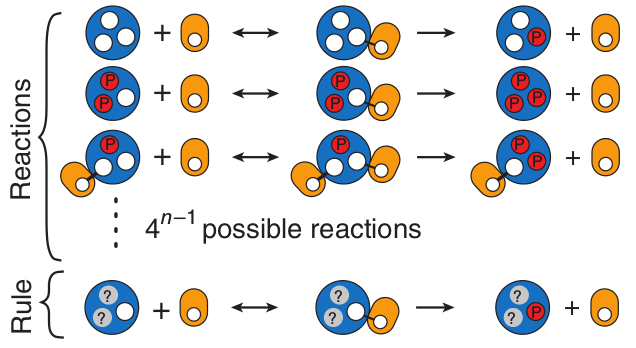
\includegraphics[scale=0.5]{pics/reaction_vs_rule}
\end{center}
\caption{bla}
\end{figure}

The rule and reaction differ in level of abstraction. In this context we mean how stringent it is, not what sort of features particular language uses. This is universal attribute for all rule-based languages -- the rule is always more abstract than it's instance -- a reaction. Then, analysis of such abstract object statically is a challenge. (cite ?) The reason is that most of the structural information is encoded in rules implicitly. For static analysis, explicit data are more suitable.

\section{Rule-based languages}

There are several rule-based languages dedicated for modeling of biological systems. Each of them uses different features and abstractions. In this chapter, we will try to highlight the key features for some representatives of them.

\subsection{Kappa}
\label{kappa}

This language was developed for modeling of protein-protein interactions. Therefore, the key feature of the language are it's so called \textit{agents} with \textit{binding sites}, which allow formation of bonds between the agents. Each binding site must be unique and at most one bond. Moreover, each site can occur in one of several pre-defined states.

The \textit{Kappa rules} are changing properties of the agents. Particularly, it might add/delete/change a bond or a state of one or multiple agents at once. Such as all the other rule-based languages, when we do not care about some context, we simply omit it. Example of a rule is in Figure~\ref{kappa-rule}.

\begin{figure}
\begin{center}
\begin{tabular}{c l}
(a) & A(bsa$\sim$\{ u, p \}) ; B(bsb$\sim$\{ a, i \}) \\
(b) & A(bsa), B(bsb$\sim$a) $\rightarrow$ A(bsa!1), B(bsb$\sim$a!1) \\
\end{tabular}
\end{center}
\caption{Example of a Kappa rule. (a) Definition of associated agents. (b) The rule itself. Note the context which has no importance for the interaction is omitted.}\label{kappa-rule}
\end{figure}

The general problem we have to face with in Kappa is too detailed description. For biological systems as defined in chapter~\ref{Rule-based basics}, it might be often hard to deal with all the bonds, especially in cases when we do not need such detail.

\subsection{BioNetGen Language}
\label{bngl}

BioNetGen Language (BNGL) is very similar to Kappa~\ref{kappa}. There are a few general differences: (1) it is allowed to define multiple binding sites with same name for an agent; (2) one binding site is allowed to have multiple bonds; (3) in the rules BNGL uses `+' and `.' for expressing reaction complex and complex of agents respectively. Example of a rule is in Figure~\ref{bngl-rule}.

\begin{figure}
\begin{center}
\begin{tabular}{c l}
(a) & A(bsa$\sim$u$\sim$p) \\
  & B(bsb$\sim$a$\sim$i) \\
(b) & A(bsa) + B(bsb$\sim$a) $\rightarrow$ A(bsa!1).B(bsb$\sim$a!1) \\
\end{tabular}
\end{center}
\caption{Example of a BGNL rule. (a) Definition of associated agents. (b) The rule itself. Note the A and B agents must first create \emph{reaction complex} denoted with `+' (i.e., they must be close to each other) and then they create \emph{complex of agents} denoted as `.' (i.e., they are physically connected).}\label{bngl-rule}
\end{figure}

\subsection{Biocham}

\subsection{PySB}

This language works as a package to Python language. The definition of models directly in the code allows to use the full syntax of Python, what dramatically increases expression power of PySB. On the other hand, it might be hard to follow abstraction which are this way possible and models themselves are hard to analyze. Moreover, the core of the language is made by translating to BGNL~\ref{bngl}.

\subsection{Chromar}

The language allows to define attributes for agents and range them over pre-defined domains. The qualitative semantics are given by rule match on multisets composed from these agents producing reaction. It is followed by standard application of the reaction (in manner of multiset operations). The language is very useful when creating a model where we need to create new distinct objects and control population of these objects.

Embedding this language to functional programming language Haskell increases its expressive power while making the ability of some analysis more expensive. Moreover, one needs to learn Haskell (at least it's basics) in order to use Chromar.

\begin{figure}
\begin{center}
A(a = x), A(a = y) $\xrightarrow[]{\text{f(x,y)}}$ A(a = x + y), A(a = y - 1) [g(x, y)]
\end{center}
\caption{Example of a Chromar rule.}\label{chromar-rule}
\end{figure}

I would like to highlight an important feature of stochastic semantics which this language offers. Compared to other rule-based languages, it is capable of specifying rates for individual reactions inherited from the rule. This is allowed by variable value bindings and type-determination between left- and right-hand-side of the rule.

However, when it comes to readability and presentation to the user, the language is not a best-fit. All the biologically relevant terms such as states must be encoded to natural numbers.

\subsection{SBML-multi package}

Systems biology Markup Language (SBML) is a standard established for systems biology. It is able to describe all necessary rule-based features and therefore it is possible to export each such language in this format. It is the most suitable format for exchange and storage of the models, but less for analysis and direct representation to the users (it is and XML format). It serves as intermediate language. 

\section{Biochemical Space}

definition of BCS, what is it good for

explanation of the format, importance of annotation

from informal BCS through definition by embedding to Kappa

why not good enough (informal)

how it was evolving

what it has common with rule-based languages, how it all started

** short intro, mention it is part of CMP !!!

BCS provides well described biological background for mathematical models of processes taking place in specific organism. Complete BCS provides a connection between existing ontologies and partial mathematical models. BCS offers a human readable format which can be easily edited in a dedicated editor and visualised on the website. First part of a BCS is represented by a set of \emph{entities} (to be compliant with process-algebraic frameworks we call entities \emph{agents}), while the second part contains \emph{rules} (abstractly represented chemical reactions defined over the set of entities). In our case study, a consortium of scientists is involved in modelling several cyanobacterial processes and in establishing of the respective BCS.

When building the BCS, emphasis is put on well-defined and complete annotations. Therefore, links to relevant ontologies must be specified for each entity and rule. Unique IDs provided by ontologies can help to automatically detect duplicities. IDs are also used to create hypertext links to related ontologies on the web, thus providing a one part of the already mentioned connection between ontologies and models. At this moment, links to KEGG, ChEBI, CyanoBase (cite) and other databases are supported. A single entity or a rule can have multiple links to several external databases. An example is presence of a particular entity in ChEBI as well as in KEGG. In the case of annotating enzymatic rules, an EC number (here acting as a descriptor of the rule mechanism behind the catalytic reaction) is associated to the enzyme via a respective KEGG ID.

The fact that most attributes in entity and rule definitions are tightly coupled with information from linked ontologies is the reason why we have started with describing annotation attributes. In the first place, one of these attributes is \emph{name}, which is taken from ontologies or follows the standard naming conventions. \emph{ID} of every entity is fixed by the consortium. KEGG ID, ChEBI ID or internal ID is used if no reasonable \emph{ID} is available. \emph{ID}s of rules are internal and assigned automatically.

An entity in our interpretation is a bounded space (a so-called \emph{compartment}) or a structural part of a specific organism. BCS covers a hierarchy of entities ranging from small molecules (\emph{atomic entities (agents)}) through composite structures (\emph{structure entities (agents)}) to large complex molecules (\emph{complex entities (agents)}). Our goal is to make BCS as simple as possible. In existing ontologies, entities residing in several different states (oxidised, reduced, etc.) are usually treated as separate entities, thus causing the total number of entities to be enormous. To reduce this complexity, the concept of \emph{states} is defined in BCS. They allow to define allowed set of states, in which an atomic agent might occur.

BCS extends the traditional concept of compartmentalisation with a hierarchy at the level of entities. A particular entity can reside in several different compartments. Additionally, \emph{classification} specifies the type of an entity in a sense of functional or structural characterisation.

An entity can be a part of a structurally more complex entity. We consider two kinds of composite entities: structure and complex entities. Structure entity represents partially specified composite species, e.g. a photosystem complex partially specified with prosthetic groups of interest. Complex entity represents fully specified composite species, e.g., a homodimer of KaiC protein.

Rules are specified by rule equations enriched with additional annotation information. When defining a rule equation, identifiers of substrates and products are used to make the notation of rules compact. Every entity appearing in a \emph{rule equation} has to be followed by the localisation operator associating it with a particular compartment. This is important especially for rules that act on both sides of a membrane. That way, a rule is always precisely localised in/inbetween compartments. A natural stoichiometric coefficient can be placed before any entity in a rule equation. Irreversible and reversible rules are distinguished by the operators `$\Rightarrow$', `$\Leftrightarrow$'. The `$+$' symbol is used as a separator between individual substrates and individual products. A rule can also have an assigned classification. Rule classification assigns a list of higher level biophysical processes in which the rule is involved. 

In some cases, emphasis on a detailed description leads to very complex BCS models. Abstraction of some processes is therefore needed to keep BCS models as simple as possible. To this end, rules expressing enzymatic reactions are considered in a simplified form. In fact, there should be at least two different rules describing an enzymatic reaction (one for a substrate binding and another for a catalytic step). Instead, since an enzyme is not affected during the reaction, it is affiliated to the rule as a \emph{modifier}. However, it is difficult to define precise meaning of a modifier in this case. We rather treat the modifier attribute informally as an entity \textit{which has to be present} for the rule to be enabled. The exact reaction mechanism of an enzyme is not always clear and therefore it is abstracted out.

Higher abstraction comes into account when several electrons play `musical chairs' inside protein complexes. The issue is that parts of processing protein complex can have different unstable states during a short period of time. When one tries to define all rules among these proteins, combinatorial explosion of the number of states of the complex arises. Not all of these combinations are biologically correct. Even when excluding biologically inadmissible cases, the number of states is still enormous. For the purpose of BCS, we introduce a solution inspired by the enzymatic rule mentioned above. We treat a protein complex as a structure entity on which structurally simpler entities change its state (not necessarily proteins) and we abstract from background processes. We can see a particular rule as a change of a state of a structure entity.

\subsection{The difference between BCS and BCSL}

It is important to realise the difference between Biochemical Space Language and Biochemical Space. 

The general goal of BCS is to provide knowledge base for mathematical models. In order to achieve that, Biochemical Space is formed by a database of biochemical entities. This allows us to describe particular objects with their attributes and properties and form space hierarchy. Each entity should be properly annotated by description and links to suitable external databases. However, entities are not enough for describing models since it requires also process hierarchy. Therefore, alongside with space hierarchy of entities, process hierarchy is build via interactive schemes. The hierarchy allows us to zoom on individual rules which present atomic operations happening on the entities.

To improve usability and verifiability of the BCS, we defined Biochemical Space Language. The language is formally defined and serves for describing the entities and the rules. It has rule-based semantics, what allows compact description of the objects. Moreover, the syntax was designed in order to be very concise and human-readable. Hence it is very suitable for our needs.

The whole BCS is defined in BCSL. This fact makes sure the entities and the rules are defined with all appropriate properties. Moreover, it helps us to relate objects from the models to BCS objects. Note that due to rule-based nature of the BCSL, in BCS there are defined only abstract objects representing types. Therefore, when relating for example an model variable to BCS entity, we might need to specify it's properties. 

Once BCS is build, we can use it to reference the models. It means to relate all the variables and reactions of the model and to entities and rules of BCS. In particular, each variable should have assigned an entity for BCS. It increases information value of the variable (due to annotation of BCS entity). Since reactions of the model are composed from its variables, this way we also rewrite general reactions to reactions written in BCSL. The result of relating all the entities is model written in BCSL. 

Model defined in BCSL has two main advantages -- formal analysis can be applied on the model and the biological meaning of the whole model is fully reconstructed.

To sum it up, BCS serves as definition domain for models written in BCSL (so called signature). It defines what can and what cannot be written in models and also increases rule compactness due to syntactic extensions. For example, some context might be omitted from the rule because it can be reconstructed from the signature.


\subsection{How is BCS accompanied with visualisation}

Best way how to present process hierarchy of BCS is via visualisation. We have employed several interactive schemes representing chosen important processes. These schemes go through abstract "higher" process to particular rules. In a scheme, a "lower" process, rule or an entity might be showed. However, the schemes might get quite complex. For this reason, a table of complete list of entities and rules is assigned to the scheme while skipping less important ones from the visualisation.


\subsection{The level of abstraction}

When describing particular process or object, we can go almost infinitely deeper into details. Even if the depth is not infinite, it deep enough to lead into state when the description larger than object itself. Imagine that you want to describe a molecule as position of each atom. You definitely need more space to store such information than the molecule itself occupies.

Therefore, when creating BCS, we choose a level of details which we do not exceed. This ensures the size of BCS will not exponentially increase with additional details. The problem might occur when we try to map a model which uses more detailed description of the system than BCS does. However, we simply allow relating multiple model objects to BCS objects and vice versa. For example, multiple model reaction might be mapped on one BCS rule denoting the fact the process represented by the rule can be described in more details by the reactions. On the other hand, model might neglect some details. Then for example, a reaction can be mapped on multiple rules with similar meaning than in previous example.

\subsection{Inclusion of BCS in SBML export (annotation)}

Since platform allows export of models in SBML format, we employed resolvable identifier links. These links are included in generated SBML file and point to appropriate rules/entities in BCS. 

\chapter{Problem formulation}

why we need something new - need of BCS by consortium, later naturally evolved into need of formal definiton

other languages didnt use suitable level of abstraction (explain why)

what was wrong before

highlight 

motivated by practical needs of ecyano (it means here it should be known from background)

Biochemical Space as described in (ref) is great idea. However, one must consider the fact that the space might get quite huge. It means keep it consistent in informal form is almost impossible. It is necessary to be able to detect inconsistency with automatic tools and enable further analysis of the space. The annotation itself is good, but with enabled formal part with all its advantages is much better. 

For this reasons we decided to improved description part of BCS by defining it formally. Many options how to define the language were available. First of all, we wanted to keep definition space as concise as is possible. Rule-based approach was the best hit, because it is capable to capture required details for biological systems while keeping the description concise. However, there are many rule-based languages and each of them is slightly different in syntactic and semantic level and also on level of abstraction. After deep research (ref prev capt), we have evaluated all existing languages as not suitable. The closest representation to the desired one (ref next section) was Kappa. That is the reason why in first iteration we have chosen translation to Kappa for definition of semantics. However, there were few aspects which were not suitable (ref).

There are several aspects which must be considered when defining new language. From syntactic point of view, we were due to keep the language as simple as possible. It was supposed to be human-readable, which in this context means easy to read, write and maintain by humans even from other disciplines than computer science. From semantic point of view, we needed a straightforward definition which would have practical use in implementation. With experiences from previous iteration, it showed that direct rule-based semantics where quite complicated mechanism of matching and replacement is used, is not very efficient. Therefore we chose indirect definition via reactions -- `practical definition' (ref formal). The level of abstraction point of view is discussed in next section.

\section{Desired abstraction level}

explain what kind of systems we need to describe

which details we dont need

and which we need

\section{What was wrong with translation to Kappa}

abstraction which were not suitable

slow implementation (cross ref)

\chapter{Formal definition}

In this chapter, we define Biochemical Space Language formally. First, we define all the required objects, then we define syntax of the language and finally give semantics to the BCSL models.

\section{Objects definition}

Let $\mathcal{N}_{A},~\mathcal{N}_{T},~\mathcal{N}_{\delta},~\mathcal{N}_{c}$ be mutually exclusive finite sets of atomic, structure, state names, and compartments, respectively.

\begin{definition}{Signature}
Atomic signature $\Sigma_{\mathtt{A}} \subseteq \mathcal{N}_{A} \times 2^{\mathcal{N}_{\delta}}$ associates atomic names with set of state names. 

Structure signature $\Sigma_{\mathtt{T}} \subseteq \mathcal{N}_{T} \times 2^{\mathcal{N}_{A}}$ associates structure names with set of atomic names. 
\end{definition}

Signatures define for an atomic name allowed set of state names and for a structure name allowed set of atomic names. The deeper meaning will be revealed after next part of definitions.

\begin{example}{Signature}\label{example:signature}
\begin{itemize}
\item An atomic signature $(S, \{u, p\})$, $(Q, \{a, i\})$
\item A structure signature $(KaiC, \{S, Q\})$
\end{itemize}
\end{example}

\noindent\rule{\textwidth}{1pt}

\begin{definition}{Atomic agent}
Atomic agent $\mathtt{A}$ is a pair $(\eta, \delta)$ where $\eta \in \mathcal{N}_{A}$ is a name and \\ $\delta~\in~\mathcal{N}_{\delta} \cup \{ \varepsilon \}$ is a state.
\end{definition}

\begin{definition}{Equivalence of atomic agents}
Let $\mathtt{A}, \mathtt{A}'$ be atomic agents. $\mathtt{A}$ is \emph{equivalent} with $\mathtt{A}'$, written $\mathtt{A} \equiv \mathtt{A}'$, iff $\eta(\mathtt{A}) \equiv \eta(\mathtt{A}') \wedge \delta(\mathtt{A}) \equiv \delta(\mathtt{A}')$.
\end{definition}

Note: maybe the definition of equivalence should be done only on names (due tu partial composition in structs).

\begin{notation}
Let $\mathds{A}$ be universe of all possible atomic agents.
\end{notation}

Atomic agents are the simplest objects used for describing biological entities. An atomic signature with the same name as the atomic agent has defines allowed states for it (with additional $\varepsilon$ state).

\begin{example}{Atomic agents}\label{example:atomic}

\begin{itemize}
\item An atomic agent $\mathtt{A}_1 = (S, u)$
\item An atomic agent $\mathtt{A}_2 = (Q, \varepsilon)$
\end{itemize}
\end{example}

Please note state $\varepsilon$ does not mean the agent is in \emph{none} state, but rather the state is unknown or not important.

\noindent\rule{\textwidth}{1pt}

\begin{definition}{Structure agent}
Structure agent $\mathtt{T}$ is a pair $(\eta, \gamma)$ where $\eta \in \mathcal{N}_{T}$ is a name and $\gamma \subseteq \mathds{A}$ is a set of atomic agents called partial composition.
\end{definition}

A structure agent represents a biochemical object that is composed from several known atomic agents provided that we know that such a composition is abstract and not necessarily complete. To incorporate such an abstraction of biological structures into our language, a structure agent is defined to be labeled with a unique name and it is constructed only from atomic agents considered in the same physical compartment.

\begin{definition}{Equivalence of structure agents}
Let $\mathtt{T}, \mathtt{T}'$ be structure agents. $\mathtt{T}$ is \emph{equivalent} with $\mathtt{T}'$, written $\mathtt{T} \equiv \mathtt{T}'$, iff $\eta(\mathtt{T}) \equiv \eta(\mathtt{T}') \wedge \forall \mathtt{A} \in \gamma(\mathtt{T}) ~\exists \mathtt{A}' \in \gamma(\mathtt{T}') : \mathtt{A} \equiv \mathtt{A}' \wedge \forall \mathtt{A}' \in \gamma(\mathtt{T}') ~\exists \mathtt{A} \in \gamma(\mathtt{T}) : \mathtt{A}' \equiv \mathtt{A}$.
\end{definition}

The key construct of a structure agent is \emph{partial composition} defined as a list of atomic agents which are considered to be relevant parts of the structure agent. We allow this list to be empty, in that case the meaning is a biological structure for which we do not know its composition.

\begin{notation}
Let $\mathds{T}$ be universe of all possible structure agents.
\end{notation}

A typical example of a structure agent is a protein where the atomic agents are individual amino acids that are of interest in the particular setting.

\begin{example}{Structure agent}\label{example:structure}
\begin{itemize}
\item A structure agent $\mathtt{T}_1 = (K, \textcolor{red}{\{}(S, p), (Q, i)\textcolor{red}{\}})$
\item A structure agent $\mathtt{T}_2 = (K, \textcolor{red}{\{}(Q, a)\textcolor{red}{\}})$
\end{itemize}
\end{example}

\noindent\rule{\textwidth}{1pt}

\begin{definition}{Complex agent}
Complex agent $\mathtt{X}$ is a pair $(\mu, \mathtt{com})$ where $\mu \in (\mathds{A} \cup \mathds{T})^n$ is a sequence, $\mathtt{com} \in \mathcal{N}_{c}$ is a compartment, and $n \in \mathbb{N}$.
\end{definition}

A complex agent represents a non-trivial composite biochemical object that is (inductively) constructed from already known biological objects. In common rule-based languages this is typically defined by introducing some kind of bonds between individual biochemical objects. In BCSL we abstract from detailed specification of bonds and we rather assume a complex as a coexistence of certain objects in a particular group. Moreover, a complex agent resides in a compartment, which gives it a space position. 

\begin{notation}
Let $\mathtt{X}$ be a complex agent. We denote length of sequence $\mu$ as $\mathtt{len}(\mathtt{X})$. 
\end{notation}

\begin{definition}{Equivalence of complex agents}\label{rule_equiv}
Let $\mathtt{X}, \mathtt{X}'$ be complexes. $\mathtt{X}$ is \emph{equivalent} with $\mathtt{X}'$, written $\mathtt{X} \equiv \mathtt{X}'$, iff $\mathtt{len}(\mathtt{X}) \equiv \mathtt{len}(\mathtt{X'}) \wedge \exists $ permutation $ \mu'(\mathtt{X}')$ of $\mu(\mathtt{X}')$ such that $\forall i~\in~[1,~n]: \mu(\mathtt{X})_i \equiv \mu'(\mathtt{X}')_i$.
\end{definition}

The key element of a complex agent is \emph{sequence} describing inductively constructed coexistence expressions from existing agents. In contrast to partial composition in structure agent, we allow replication at the level of sequence (an agent of a certain name can appear more than once in a sequence).

\begin{notation}
Let $\mathds{X}$ be universe of all possible complex agents. Moreover, we denote $\mathds{U} = \mathds{A} \cup \mathds{T} \cup \mathds{X}$ as universe of all possible agents.
\end{notation}

\begin{example}{Complex}\label{example:complex}

\begin{itemize}
\item A complex $\mathtt{X} = (\textcolor{green}{(}(K, \textcolor{red}{\{}(S, p), (Q, i)\textcolor{red}{\}}), (S, p)\textcolor{green}{)}, cytosol)$
\end{itemize}
\end{example}

The complex agents have very important role in the language. In the rules defined in following, we can always use only complexes. It means, an atomic or structure agent cannot exist on its own, it must be encapsulated in a complex -- it might have only one item in its sequence. Moreover, this guarantees each atomic and structure agent has indirectly given space location -- the compartment.

\noindent\rule{\textwidth}{1pt}

\begin{definition}{Rule}

Rule $\mathtt{R}$ is a 5-tuple $(\chi, \omega, \mathtt{I}, \mathtt{map}, \mathtt{Indices})$ where:

\begin{itemize}
\item $\chi \in \mathds{X}^n$ is a sequence of complexes,
\item $\omega \in (\mathds{A} \cup \mathds{T})^m$ is a sequence of atomic and structure agents,
\item $\mathtt{I} \in \{ 1, \ldots, n \}$ is an index determining start of right-hand-side,
\item $\mathtt{map} \in \mathbb{N}^m$ is an index map between $\omega$ and $\chi$,
\item $\mathtt{Indices} \subseteq (\{-\} \cup \mathbb{N})^2$ is an index map between agents from left- and right-hand side (always sorted lexicographically such that $'-' > i$ for every $i \in \mathbb{N}$)
\end{itemize}

where $n, m \in \mathbb{N}$.
\end{definition}

As can be seen, rule is quite a complicated structure. The reason is the practical definition of semantics which in following section (ref). Also, it is necessary to capture relationship between left- and right-hand side of the rule. This is done by enumerating all atomic and structure agents in $\omega$ and consequently creating index map between the agents in $\mathtt{Indices}$. Another index map $\mathtt{map}$ serves for relating agents from $\omega$ back to original sequence of complexes $\chi$. Finally, by index $\mathtt{I}$ we determine the end of left-hand side of the rule.

\begin{notation}
Let $\mathds{R}$ be universe of all possible rules.
\end{notation}

\begin{example}{Rule}\label{example:rule}

\begin{itemize}
\item 
$\chi = \begin{bmatrix}
(\textcolor{green}{(} (K, \textcolor{red}{\{}(S, u)\textcolor{red}{\}}), (B, \textcolor{red}{\emptyset}) \textcolor{green}{)}, cyt),\\

(\textcolor{green}{(} (C, \textcolor{red}{\emptyset}), (D, i) \textcolor{green}{)}, cyt),\\

(\textcolor{green}{(} (A, \varepsilon) \textcolor{green}{)}, cyt),\\

(\textcolor{green}{(} (K, \textcolor{red}{\{}(S, p)\textcolor{red}{\}}), (B, \textcolor{red}{\emptyset}), (C, \textcolor{red}{\emptyset}) \textcolor{green}{)}, cyt),\\

(\textcolor{green}{(} (D, a), (A, \varepsilon) \textcolor{green}{)}, cyt),\\

(\textcolor{green}{(} (H, u) \textcolor{green}{)}, cyt)  
\end{bmatrix}$

\item $\omega = \begin{bmatrix}
(K, \textcolor{red}{\{}(S, u)\textcolor{red}{\}}), (B, \textcolor{red}{\emptyset}), (C, \textcolor{red}{\emptyset}), \\
(D, i), (A, \varepsilon), (K, \textcolor{red}{\{}(S, p)\textcolor{red}{\}}), \\
(B, \textcolor{red}{\emptyset}), (C, \textcolor{red}{\emptyset}), (D, a), (A, \varepsilon), (H, u)
\end{bmatrix}$

\item $\mathtt{I} = 3$
\item $\mathtt{map} = (2,4,5,8,10,11)$
\item $\mathtt{Indices} = [ (1,6) ; (2,7) ; (3,8) ; (4,9) ; (5,10) ; (-,11) ] $
\end{itemize}
\end{example}

\noindent\rule{\textwidth}{1pt}

\begin{definition}{Reaction}

Reaction $\mathtt{r}$ is a pair $(\mathtt{seq}, \mathtt{I})$ where:

\begin{itemize}
\item $\mathtt{seq} \in \mathds{X}^n$ is a sequence of complexes,
\item $\mathtt{I} \in \{ 1, \ldots, n \}$ is an index determining start of right-hand-side
\end{itemize}

where $n, m \in \mathbb{N}$.
\end{definition}

Reaction is similar structure than rule, but much simpler. The reaction is just mediate format for giving semantics to BCSL models and it only holds information about complex contents of the rule.

\begin{notation}
We denote left-hand-side of the reaction $(\mathtt{seq}_0, \ldots, \mathtt{seq}_{\mathtt{I}-1})$ as $LHS(\mathtt{r})$ and right-hand-side of the reaction$(\mathtt{seq}_\mathtt{I}, \ldots, \mathtt{seq}_n)$ as $RHS(\mathtt{r})$.
\end{notation}

\noindent\rule{\textwidth}{2pt}

\section{Syntax}

In this section, we define grammar for the BCSL. As proposed in (ref), the syntax must be simple and readable. It was already defined in (cite), here we give just simplified version of the definition.

\begin{definition}{Grammar}
\begin{center}
\begin{tabular}{ l l }
atomic expression & $\alpha ::= \eta\{s\} ~|~ \eta$\\
 & $\eta ::= n \in \mathcal{N}_{A}$ \\
 & $s ::= n \in \mathcal{N}_{\delta}$\\
 & \\
structure expression & $\tau ::= \eta(\gamma) ~|~ \eta$\\
 & $\gamma ::= \alpha_1, \ldots, \alpha_k$ \\
 & $\eta ::= n \in \mathcal{N}_{T}$\\
 & \\
complex expression & $\Gamma ::= \beta_1~.~\ldots~.~\beta_k :: c$\\
 & $\alpha_i ::= \alpha ~|~ \tau$\\
 & $c ::= n \in \mathcal{N}_{c}$\\
 & \\
rule expression & $\rho ::= \Gamma_1 + \ldots + \Gamma_n \Rightarrow \Gamma_{n+1} + \ldots + \Gamma_m $
\end{tabular}

\end{center}
where $m,n \in \mathbb{N}_0 \wedge m > n \wedge m + n \neq 0$ and $k \in \mathbb{N}$.
\end{definition}

\begin{example}{Syntax}\label{example:syntax}

Examples of agents, complexes and rules given in previous examples:

\begin{itemize}
\item $\mathtt{A}_1$ is written as $S\{u\}$, $\mathtt{A}_2$ is written as $Q$ (Example~\ref{example:atomic}),

\item $\mathtt{T}_1$ is written as $K(S\{p\}, Q\{i\})$, $\mathtt{T}_2$ is written as $K(Q\{A\})$ (Example~\ref{example:structure}),

\item $\mathtt{X}$ is written as $K(S\{p\}, Q\{i\}).S\{p\}::cytosol$ (Example~\ref{example:complex}),

\item rule $\mathtt{R}$ is written as (Example~\ref{example:rule}):
\end{itemize}

\noindent {\small $K(S\{u\}).B::cyt + C.D\{i\}::cyt + A::cyt \Rightarrow K(S\{p\}).B.C::cyt + D\{a\}.A::cyt + H\{u\}::cyt$}
\end{example}

\noindent\rule{\textwidth}{1pt}

\section{BCSL model}

\begin{definition}{BCSL model}
We define BCSL model $\mathds{M}$ as 4-tuple $(\mathcal{R}, \Sigma_\mathtt{A}, \Sigma_\mathtt{T}, \mathtt{init})$ where $\mathcal{R}$ is set of rule expressions, $\Sigma_\mathtt{A}$ is atomic signature, $\Sigma_\mathtt{T}$ is structure signature, and $\mathtt{init}$ is initial multiset of complex expressions $\Gamma$.
\end{definition}

\noindent\rule{\textwidth}{1pt}

\section{Additional definitions}

Before we proceed, there are few necessary definitions.

\begin{definition}{Tuples concatenation}

Let $X = (x_1, \ldots, x_n), Y = (y_1, \ldots, y_m)$ be two tuples for some $n, m \in \mathbb{N}$. Concatenation of two tuples, written $X \mdoubleplus Y$, is defined as:

\begin{center}
$X \mdoubleplus Y = (x_1, \ldots, x_n, y_1, \ldots, y_m)$.
\end{center}
\end{definition}

\begin{definition}{Sum of concatenations}

Let $T = (T_1, T_2, \ldots, T_n)$ be sequence of tuples where $\tau_i = (x_{i_1}, \ldots, x_{i_m})$. Concatenation of sequence of tuples $\Xi_{i=1}^n T_i$ is defined as:

\begin{center}
$\Xi_{i=1}^n T_i = T_1 \mdoubleplus T_2 \mdoubleplus \ldots \mdoubleplus T_n $
\end{center}
\end{definition}

\begin{definition}{Reassembly}

Let $Y$ be a set of tuples of particular form, where each $y \in Y$ has form $((a_1, b_1), (a_2, b_2), \ldots, (a_n, b_n))$. Reassembly of set $Y$ is a set of tuples $X$ where each $x \in X$ has form $(a_1, a_2, \ldots, a_n, b_1, b_2, \ldots,  b_n)$. formally

\begin{center}
$\mathtt{reassembly}(Y) = \{~  x ~|~ y \in Y \wedge x = \Xi_{i=1}^{|y|} y_{i_1} \mdoubleplus \Xi_{i=1}^{|y|} y_{i_2} ~\}$
\end{center}
\end{definition}

\begin{definition}{Difference of partial compositions}

Let $\gamma, \gamma'$ be two partial compositions. We define difference of these two sets on names of its atomic agents as following:

\begin{center}
$\gamma \ominus \gamma' \Leftrightarrow \{ \mu_\alpha ~|~ \exists \mathtt{A}: (\mathtt{A} \in \gamma \wedge \mu(\mathtt{A}) \equiv \mu_\alpha ) \wedge \not\exists \mathtt{A}': (\mathtt{A}' \in \gamma' \wedge \mu(\mathtt{A}') \equiv \mu_\alpha)\}$
\end{center}
\end{definition}

\begin{definition}{Difference of partial composition and structure signature}

Let $\mathtt{T}$ be a structure agent. Next, let $\gamma(\mathtt{T})$ be its partial composition and $\Sigma_T(\mathtt{T})$ appropriate signature. We define difference of these two sets on names of atomic agents as following:

\begin{center}
$\gamma(\mathtt{T}) \ominus \Sigma_T(\mathtt{T}) \Leftrightarrow \{ \mu_\Sigma ~|~ \mu_\Sigma \in \Sigma_T(\mathtt{T}) \wedge \not\exists \mathtt{A}: (\mathtt{A} \in \gamma(\mathtt{T}) \wedge \mu(\mathtt{A}) \equiv \mu_\Sigma)\}$
\end{center}
\end{definition}

\section{Semantic function}

In the previous sections, we defined BCSL objects and BCSL model. Now, we need to connect them such that we give semantic meaning to the model $\mathds{M}$. For this purpose, we define semantic function $\mathtt{F}$. It is defined recursively for a model $\mathds{M}$ according to expression given as argument:

\begin{center}
\begin{tabular}{ r c l}
$\mathtt{F} \llbracket ~\mu~ \rrbracket$ & = &
    $\begin{cases}
    (\mu, \epsilon) \in \mathds{A} ~\ldots~ \mu \in \Sigma_{A}\\
    (\mu, \emptyset) \in \mathds{A} ~\ldots~ \mu \in \Sigma_{T}\\
    \end{cases}
    $\\
 & & \\
$\mathtt{F} \llbracket ~\mu\{s\}~ \rrbracket$ & = & $(\mu, s) \in \mathds{A}$\\
 & & \\
$\mathtt{F} \llbracket ~\mu(\mathtt{a}_1, \ldots, \mathtt{a}_n)~ \rrbracket$ & = &
$(\mu, \{~ \mathtt{F} \llbracket \mathtt{a}_1 \rrbracket, \ldots, \mathtt{F} \llbracket \mathtt{a}_n \rrbracket ~\}) \in \mathds{T}$\\
 & & \\
$\mathtt{F} \llbracket ~\alpha_1~.~\ldots~.~\alpha_n :: c~ \rrbracket$ & = &
$(~(\mathtt{F} \llbracket ~\alpha_1~ \rrbracket, \ldots, \mathtt{F} \llbracket ~\alpha_n~ \rrbracket), ~c~) \in \mathds{X}$\\
 & & \\
$\mathtt{F} \llbracket ~\Gamma_1 + \ldots + \Gamma_n \Rightarrow \Gamma_{n+1} + \ldots + \Gamma_m~ \rrbracket$ & = &
$(\chi, \omega, \mathtt{I}, \mathtt{map}, \mathtt{Indices}) \in \mathds{R}$~ such that:\\
\end{tabular}
\end{center}

\begin{center}
\begin{itemize}
\item $\chi = (\mathtt{F} \llbracket ~\Gamma_1~ \rrbracket, \ldots, \mathtt{F} \llbracket ~\Gamma_n~ \rrbracket, \mathtt{F} \llbracket ~\Gamma_{n+1}~ \rrbracket, \ldots, \mathtt{F} \llbracket ~\Gamma_m~ \rrbracket)$,
\item $\omega = \Xi_{i=1}^{|\chi|} \mu(\chi_i)$,
\item $\mathtt{I} = n$,
\item $\mathtt{map} = (J_1, \ldots, J_m): J_i = \sum_{y=1}^{i} | \mu(\chi_y) |$,
{\small
\item \begin{tabular}{l l}

& \hspace*{-0.3cm} $\{~ (i,j) ~|~ i \in [1, \mathtt{map}(\mathtt{I})] \wedge j \in [\mathtt{map}(\mathtt{I}), |\omega|] \wedge |i-j| \equiv \mathtt{map}(\mathtt{I})~\} ~\cup$ \\

\hspace*{-0.3cm}$\mathtt{Indices} =$ & \hspace*{-0.3cm} $\{~ (i, -) ~|~ i \in [k, \mathtt{map}(\mathtt{I})] \wedge k = |~ \{ \mathtt{map}(\mathtt{I}) + 1, \ldots, | \alpha | \} ~| ~\} ~\cup$\\

& \hspace*{-0.3cm} $ \{~ (-, j) ~|~ j \in [k, |\alpha|] \wedge k = 2 * \mathtt{map}(\mathtt{I}) ~\}$
\end{tabular}
\\}

\end{itemize}
\end{center}

Please note by applying semantic function $\mathtt{F}$ on examples from Example~\ref{example:syntax}, we obtain agents (resp. complex or rule) from appropriate referenced examples. Moreover, semantic function work \emph{only} on BCSL object and rules well-defined by the given grammar (ref).


\noindent\rule{\textwidth}{2pt}

\section{Ground forms}

Ground form represents appending context to agents according to signature (we assume signature is always available and therefore we omit it in ground from function arguments).

Objects are transformed to their ground forms by ground form function $\mathcal{G}$ defined as following:

\begin{center}
\begin{tabular}{ c c l }
Object type & Basic form & Ground form \\
\hline
 & & \\
$\mathds{A}$ & $\mathcal{G}((\mu, \epsilon))$ & $\{~ (\mu, \delta) ~|~ \delta \in \Sigma_A(\mu) ~\}$\\
 & $\mathcal{G}((\mu, \delta))$ & $\{~(\mu, \delta) ~\}$\\
 & & \\
 \hline
 & & \\
$\mathds{T}$ & $\mathcal{G}((\mu, \gamma))$ & $\{~ (\mu, \gamma_\alpha) ~|~ \gamma_\alpha \equiv \gamma \cup \gamma_\Sigma \wedge \gamma_\Sigma = \{~ \mathtt{A}_1, \ldots, \mathtt{A}_n ~\} \wedge$\\
 & & $\wedge~ \mathtt{A}_i \in \mathcal{G}((\mu, \emptyset)) \wedge \mu \in \gamma \ominus \Sigma_T(\mathtt{T}) ~\}$ \\
 & & \\
 \hline
 & & \\
$(\mathds{A} \cup \mathds{T})^2$ & $\mathcal{G}((\beta, \beta'))$ & $\{~ (\beta_\alpha, \beta_\alpha') ~|~ \beta_\alpha \in \mathcal{G}(\beta) \wedge \beta'_\alpha \in \mathcal{G}(\beta') \wedge$\\
 & & $\wedge~ \gamma(\beta_\alpha) \ominus \gamma(\beta) \equiv \gamma(\beta'_\alpha) \ominus \gamma(\beta') ~\} $ \\
 & & \\
 \hline
 & & \\
$\mathds{R}$ & $\mathcal{G}(\mathtt{R})$ & $ \bigotimes \mathcal{G}(\mathtt{Indices})^* $ \\
 & $\mathcal{G}(\mathtt{Indices})$ & $(~\mathcal{G}(\omega(i), \omega(j)) ~|~ (i,j) \in \mathtt{Indices})$\\
 
\end{tabular}
\end{center}

where $\bigotimes \mathcal{G}(\mathtt{Indices})^*$ is Cartesian product of sets inside of tuple $\mathcal{G}(\mathtt{Indices})$.

\noindent\rule{\textwidth}{2pt}

\section{Construction of reactions}
\label{Generating reactions}

Given a rule $\mathtt{R}$, we can produce appropriate reactions using ground forms and subsequent application of reassembly operation.

\begin{definition}{Construction of reactions}\label{generate_reactions}
\hspace*{-0.8cm}\begin{tabular}{ r l }
$\mathtt{Reactions}(\mathtt{R}) =$ & $\{~ \mathtt{r}(\mathtt{seq}, \mathtt{I}) ~|~ y \in \mathtt{reassembly}(\mathcal{G}(\mathtt{R})) ~\}$,\\

where $\mathtt{seq} =$ & $ \big(\mathtt{X}(y(0, \ldots, \mathtt{map}(0) - 1), \mathtt{com}(\chi(0))),$ \\

& $\mathtt{X}(y(\mathtt{map}(0), \ldots, \mathtt{map}(1) - 1), \mathtt{com}(\chi(1))), $\\

& \ldots,\\

& $\mathtt{X}(y(\mathtt{map}(|\mathtt{map}| - 1]), \ldots, \mathtt{map}(|\mathtt{map}|) - 1, \mathtt{com}(\chi(|\mathtt{map}|)))\big) $\\

and $ \mathtt{I} \in \mathtt{R}$ & and $\chi \in \mathtt{R}$ and $\mathtt{map} \in \mathtt{R}.$\\
\end{tabular}
\end{definition}

\noindent\rule{\textwidth}{1pt}

\section{Chemical Reaction Networks}

\begin{definition}{Chemical Reaction Model (CRN)}
\label{crn}
Chemical Reaction Model $\mathcal{M}$ is a triple $(\mathfrak{R}, \vv{\nu}, \pi)$ such that $\mathfrak{R} \subseteq \mathbb{Z}^n$ is set of reactions, $\vv{\nu} \in \mathbb{N}_0^n$ is initial vector, and $\pi \in \mathds{X}^n$ is vector of reference complexes for some $n \in \mathbb{N}$.
\end{definition}

Chemical Reaction Model is a simple model, where reactions and initial state are vectors over integers. Moreover, there is a reference vector of complex agents, which servers for identifying underlaying agents behind the integers (according to particular position in vectors).

\begin{notation}\label{nonnegative}
We denote $N(\vv{\nu}) ~\emph{iff}~ \forall i \in \vv{\nu}: i \in \mathbb{N}_0$.
\end{notation}

By Notation~\ref{nonnegative} we denote the fact that a vector is formed only by non-negative integers.

\begin{definition}{Reaction application}

Reaction application $\rho$ is a relation $\rho \subseteq \mathbb{N}_0^n \times \mathbb{Z}^n \times \mathbb{N}_0^n$ such that 
\begin{center}
$(\vv{\upsilon}, \vv{\mathtt{r}}, \vv{\mathtt{u}}) \in \rho$ $\Leftrightarrow$ $\vv{\mathtt{u}} = \vv{\upsilon} + \vv{\mathtt{r}} \wedge N(\vv{\mathtt{u}})$.
\end{center}
\end{definition}

Note some values in reactions might be negative. When applying reaction on state, the resulting state cannot contain any negative values (negative number of entities does not give biological sense). Therefore, application is allowed only if the resulting vector contains non-negative values.

\begin{definition}{CRN semantics}
Let $\mathcal{M}$ be a Chemical Reaction Model. The quantitative semantics are given in terms of a discrete-states produced by iterative reaction application on initial vector $\vv{\nu}$ and all consequently created state vectors. This way we obtain an LTS (ref).
\end{definition}

CRN semantics might lead to possibly infinite LTS. This process can be limited by a global bound, which makes sure the produced LTS is finite (ref).

\noindent\rule{\textwidth}{1pt}

\section{Production of model}

In previous sections we defined all what was required to actually create Chemical Reaction Model (Definition~\ref{crn}) from a BCSL model. This procedure is necessary in order to allow operational semantics to be applied.

\begin{definition}{Reference vector}\label{reference_vector}

Reference vector $\pi$ is a tuple of all possible unique complexes constructed from reactions of model $\mathds{M}$ as following:

\begin{center}
$$\Pi = \{~ \mathtt{X} ~|~ \mathtt{X} \in \mathtt{seq}(\mathtt{r}) \wedge \mathtt{r} \in \bigcup_{\mathtt{R} \in \mathcal{R}} \mathtt{Reactions}(\mathtt{R}) ~\} $$
\end{center}

\noindent Then, reference vector $\pi$ is just chosen random order of the set $\Pi$.

\end{definition}

\begin{definition}{Multiset to vector translation}\label{state_to_vector}
Translation of multiset $\mathtt{S} \subseteq \mathds{X}$ to vector is defined as following:
\begin{center}
$\lambda(\mathtt{S}, \pi) = (a_1, a_2, \ldots, a_n)$ such that 
$a_i$ =
  $\begin{cases}
  |\mathtt{S}(\pi_i)| & \ldots~~~~ \pi_i \in \mathtt{S}\\
  0 & \ldots~~~~ \pi_i \not\in \mathtt{S}\\
  \end{cases}
  $
\end{center}
\hspace{15pt} where $n = |\pi|$ and $|\mathtt{S}(\pi_i)|$ is number of occurrences of agent $\pi_i$ in the multiset $\mathtt{S}$.
\end{definition}

Let $\mathds{M} = (\mathcal{R}, \Sigma_\mathtt{A}, \Sigma_\mathtt{T}, \mathtt{init})$ be a BCSL model. In order to construct Chemical Reaction Model $\mathcal{M} = (\mathfrak{R}, \vv{\nu}, \pi)$ from the model $\mathds{M}$, we need to apply the following steps:

\begin{enumerate}
\item generate reactions for all rules $\mathtt{F}(\mathtt{R}) \in \mathcal{R}$ (Definition~\ref{generate_reactions}),
\item construct reference vector $\pi$ (Definition~\ref{reference_vector}),
\item create initial vector $\vv{\nu}$ from initial multiset $\mathtt{S}$ constructed as $\mathtt{S} = \{ \mathtt{X} ~|~ \mathtt{X} = \mathtt{F}(\Gamma) \wedge \Gamma \in \mathtt{init} \}$ (Definition~\ref{state_to_vector}),
\item construct set of vector reactions $\mathfrak{R}$ from the set reactions, where individual vector reaction $\vv{r}$ is created from a reaction $\mathtt{r}$ as following:

\begin{center}
$\vv{r} = \lambda(RHS(\mathtt{r}), \pi) - \lambda(LHS(\mathtt{r}), \pi)$
\end{center}

\end{enumerate}

In order to accomplish the process of giving semantics to an BCSL model, it is necessary to note how we revive information which is missing in produced LTS. This procedure is quite straightforward since we still have define reference vector $\pi$. Similarly as we translated multisets of BCSL agents to vectors (Definition~\ref{state_to_vector}), we can apply a reverse procedure, when we build a multiset of agents from a vector according to the reference vector $\pi$. This is how we obtain an LTS as described in (ref).  

\section{Syntactic extensions}

We define several syntactic extensions for better readability of the rules. Note that each rule in a extended form can be always translated to basic form defined above. All rules containing the following extensions must be converted to basic form before semantics can be applied.

For better demonstration, we give running example, which will go through all syntactic extensions. Please note there is no biological sense of the model, it has only demonstrative purpose.

\begin{runningExample}{The example model $\mathds{M}$}
\label{run1}

\noindent Definition of rules $\mathtt{R}$:
{\small
\begin{enumerate}
\item $KaiC(S\{u\}, T).KaiC(S, T).KaiC(S, T)::cyt \Rightarrow $

$\Rightarrow KaiC(S\{p\}, T).KaiC(S, T).KaiC(S, T)::cyt$

\item $KaiC(S\{u\}, T).KaiB::cyt \Rightarrow KaiC(S\{p\}, T).KaiB::cyt$
\item $KaiC(S, T)::cyt + KaiC(S, T)::cyt + KaiC(S, T)::cyt \Rightarrow$ 

$ \Rightarrow KaiC(S, T).KaiC(S, T).KaiC(S, T)::cyt$

\item $KaiC(S, T).KaiC(S, T).KaiC(S, T)::cyt \Rightarrow $

$\Rightarrow KaiC(S, T)::cyt + KaiC(S, T)::cyt + KaiC(S, T)::cyt$
\end{enumerate}
}

\noindent Definition of $\Sigma_\mathtt{A}$:
\begin{enumerate}
\item $(S, \{ u, p \})$,
\item $(T, \{ a, i \})$
\end{enumerate}

\noindent Definition of $\Sigma_\mathtt{T}$:
\begin{enumerate}
\item $(KaiC, \{ S, T \})$,
\item $(KaiB, \emptyset)$
\end{enumerate}

\noindent We omit $\mathtt{init}$ definition just for simplicity of the example.
\end{runningExample}

\subsection{Omitting context in partial composition.}

It is possible to omit all partial compositions which contain a unspecified atomic agents. Such agent does not give any additional information and whole partial composition can be reconstructed from signature.

\begin{runningExample}{The example model $\mathds{M}$}
\label{run1}

\noindent Definition of rules $\mathtt{R}$:
{\small
\begin{enumerate}
\item $KaiC(S\{u\}).KaiC.KaiC::cyt \Rightarrow KaiC(S\{p\}).KaiC.KaiC::cyt$
\item $KaiC(S\{u\}).KaiB::cyt \Rightarrow KaiC(S\{p\}).KaiB::cyt$
\item $KaiC::cyt + KaiC::cyt + KaiC::cyt \Rightarrow KaiC.KaiC.KaiC::cyt$
\item $KaiC.KaiC.KaiC::cyt \Rightarrow KaiC::cyt + KaiC::cyt + KaiC::cyt$
\end{enumerate}
}
\end{runningExample}

This syntactic extension bring lot of readability to the syntax while preserving all information in context of the model $\mathds{M}$.

\subsection{Complex signature}

We extend model definition by complex signature $\Sigma_\mathtt{X}$ on syntactic level. In this signature, there are defined aliases for valid complex agent expressions. Then, simple \emph{replace} method is used to substitute original expression by the alias.

\begin{runningExample}{The example model $\mathds{M}$}\label{run1.1}

\noindent Definitions of complex signatures:
\begin{enumerate}
\item $KaiC3::cyt = KaiC.KaiC.KaiC::cyt$
\item $KaiBC::cyt = KaiC.KaiB::cyt$
\end{enumerate}

\noindent Definition of rules $\mathtt{R}$:
{\small
\begin{enumerate}
\item $KaiC(S\{u\}).KaiC.KaiC::cyt \Rightarrow KaiC(S\{p\}).KaiC.KaiC::cyt$
\item $KaiC(S\{u\}).KaiB::cyt \Rightarrow KaiC(S\{p\}).KaiB::cyt$
\item $KaiC::cyt + KaiC::cyt + KaiC::cyt \Rightarrow KaiC3::cyt$
\item $KaiC3::cyt \Rightarrow KaiC::cyt + KaiC::cyt + KaiC::cyt$
\end{enumerate}
}

\end{runningExample}

As can be seen, in this stage the complex signature has it limitations. Once a context is specified, the alias cannot be used anymore. We will resolve this problem in following extensions.

\subsection{Directions}

We allow rules to be bi-directional -- it is just a shortcut for two rules and it can be converted to basic rule form. A rule $\mathtt{R} = \lambda ~\Leftrightarrow~ \rho$ might be written as two rules $\mathtt{R}_1 = \lambda ~\Rightarrow~ \rho$ and $\mathtt{R}_2 = \rho ~\Rightarrow~ \lambda$.

\begin{runningExample}{The example model $\mathds{M}$}\label{run2}
\noindent Definition of rules $\mathtt{R}$:
{\small
\begin{enumerate}
\item $KaiC(S\{u\}).KaiC.KaiC::cyt \Rightarrow KaiC(S\{p\}).KaiC.KaiC::cyt$
\item $KaiC(S\{u\}).KaiB::cyt \Rightarrow KaiC(S\{p\}).KaiB::cyt$
\item $KaiC::cyt + KaiC::cyt + KaiC::cyt \Leftrightarrow KaiC3::cyt$
\end{enumerate}
}
\end{runningExample}

\noindent Definition of rules 3 and 4 from Running example~\ref{run1.1} was replaced by one bi-directional rule (Running example~\ref{run1.1}, rule 3).

\subsection{Stoichiometry}

For a rule of form $(\alpha_1, \alpha_2, \ldots, \alpha_n) \Rightarrow \alpha_1.\alpha_2.~\ldots~.\alpha_n$, we might reorder both sides such that we get noncrossing partition $\mathcal{P}([1,\ldots,n])$ from its indices such that $\forall \mathcal{P}_i: \forall x,y \in \mathcal{P}_i: \alpha_x \equiv \alpha_y$ and $\forall \alpha_x \in \mathcal{P}_i \forall \alpha_y \in \mathcal{P}_j: \alpha_x \not\equiv \alpha_y$. Each $\mathcal{P}_i$ forms equivalence groups $\mathcal{G}_\equiv$ of \textit{k} rule agents.

Such a new rule is equivalent with the original rule what follows from rules equivalence definition (Definition~\ref{rule_equiv}).

For side $\mathtt{s} = (\alpha_1, \alpha_2, \ldots, \alpha_n)$ of the reordered rule we enrich $\alpha$ context to pair $(\iota, \alpha)$ with $\iota = 1$. However, some $\alpha${\footnotesize s} in $\mathtt{s}$ might be equivalent and then they belong to an equivalence group $\mathcal{G}_\equiv$. Each of these groups $\mathcal{G}_\equiv$ might be written as one pair $(\iota, \alpha_m)$ where $\iota = |\mathcal{G}_\equiv|$ for some $\alpha_m \in \mathcal{G}_\equiv$.

Note that this process is fully reversible, so agent enumeration in basic form can be easily reconstructed.

\begin{runningExample}{The example model $\mathds{M}$}\label{run3}
\noindent Definition of rules $\mathtt{R}$:
{\small
\begin{enumerate}
\item $KaiC(S\{u\}).KaiC.KaiC::cyt \Rightarrow KaiC(S\{p\}).KaiC.KaiC::cyt$
\item $KaiC(S\{u\}).KaiB::cyt \Rightarrow KaiC(S\{p\}).KaiB::cyt$
\item $3~KaiC::cyt \Leftrightarrow KaiC3::cyt$
\end{enumerate}
}
\end{runningExample}

\noindent Definition of rule 3 from Running example~\ref{run2} was replaced by using stoichiometry.

\subsection{Locations}

Probably most complex syntactic extension is application of locations. The localisation operator is intended for allowing an alternative way of expressing the hierarchically constructed agents. The main idea is to allow zooming into individual parts of complex and structure agents.

We define necessary condition which must hold when semantic function $\mathtt{F}$ is applied on individual agents. This notation is allowed only when the conditions hold.

\begin{definition}{Locations conditions.}\label{locations:conditions}

\begin{enumerate}
 \item $\mathtt{A}::\mathtt{T}$ $\Leftrightarrow$ there exists $\mathtt{A}' \in \gamma(\mathtt{T})$ such that $\mathtt{A} \lhd \mathtt{A}'$,

\item $\mathtt{A}::\mathtt{X}$ $\Leftrightarrow$ there exists $\mathtt{A}' \in \mu(\mathtt{X})$ such that $\mathtt{A} \lhd \mathtt{A}'$,

\item $\mathtt{T}::\mathtt{X}$ $\Leftrightarrow$ there exists $\mathtt{T}' \in \mu(\mathtt{X})$ such that $\mathtt{T} \lhd \mathtt{T}'$.
\end{enumerate}
\end{definition}

For each pair of agents $(\alpha, \beta)$ with allowed `::' operator between them $\alpha :: \beta$, we can construct just one agent $\beta'$ without the operator by taking most-left agent $\alpha'$ from full (resp. partial) composition of the agent $\beta$ such that it is \emph{compatible with} the agent $\alpha$ ($\alpha' \lhd \alpha$). Then, agent $\alpha'$ is simply replaced by agent $\alpha$ and agent $\beta'$ is constructed.

\begin{runningExample}{The example model $\mathds{M}$}\label{run4}
\noindent Definition of rules $\mathtt{R}$:
{\small
\begin{enumerate}
\item $S\{u\}::KaiC::KaiC3::cyt \Rightarrow S\{p\}::KaiC::KaiC3::cyt$
\item $S\{u\}::KaiC::KaiBC::cyt \Rightarrow S\{p\}::KaiC::KaiBC::cyt$
\item $3~KaiC::cyt \Leftrightarrow KaiC3::cyt$
\end{enumerate}
}
\end{runningExample}


\noindent Definition of rules 1 and 2 from Running example~\ref{run1} was replaced using locations.

You can see localisation operator allowed us to fully use the complex signatures.

\subsection{Variables}

In the Running example~\ref{run4} there is still space for syntax reduction. Rule 1 and 2 are very similar except context of complex they take place in. Therefore, we will substitute this context with a variable with given domain.

In a rule, one rule agent might be referenced using variable $\upsilon$ as a set of rule agents it can be replaced with. Such a rule agent is referenced as $?X$. Moreover, in case when a $?X$ is used in a location, it must hold conditions from Definition~\ref{locations:conditions}.

Once again, each rule associated with variable can be easily rewritten as several rules where variable is replaced with agent from set of agents attached to the variable. Please note only one variable can be used per rule.

\begin{runningExample}{The example model $\mathds{M}$}\label{run5}
\noindent Definition of rules $\mathtt{R}$:
{\small
\begin{enumerate}
\item $S\{u\}::KaiC::~?X::cyt \Rightarrow S\{p\}::KaiC::~?X::cyt ~;~ ?X = \{KaiC3, KaiBC\}$
\item $3~KaiC::cyt \Leftrightarrow KaiC3::cyt$
\end{enumerate}
}
\end{runningExample}

\noindent Definition of rules 1 and 2 from Running example~\ref{run4} was replaced as a single rule using a variable.

This is final syntactic extension. Compared to original model (Running example~\ref{run1}), the resulting model is much more concise and readable. More examples can be seen in chapter (ref case study).

\chapter{Analysis}

* discuss problems, pros and cons, etc

multisets compared to graphs (isomorphisms) - other languages

In the previous chapters, we defined BCS language itself. From the provided examples and case study (ref) it should be clear that it provides concise and readable notation when it comes to describing biological systems. Moreover, accompanied with relevant annotation information, it is suitable for building huge models.

However, descriptive properties are not enough for using computational methods in order to analyse particular processes. In this chapter we describe basic approaches we employ for our language and propose several methods which could be potentially used in context of static analysis.

We distinguish two general approached in model analysis -- dynamic and static. Dynamic analyses are enabled by some form of executing the model. It requires either enumerating all possible scenarios of model's behavior (so called state space) or applying assumptions in order to calculate average behavior (simulation). On the other hand, static analyses provide information without execution of the model, just by investigating it's structure. Both approaches require to build particular mechanisms which enable application of the analyses.

\section{Dynamic analyses}

briefly explain how (non)deterministic simulations work, give citations

 - difference, when which of them can be used, explain biological meaning behind
 - all the distributions etc

problem of model checking, why it is problem, how it works (see my BT) 

 - we focus on reachability in general in this theses, later could be extended to entire model checking problem

such as simulation, model checking (reachability)

explain that state space might be unbounded, disscuss what does it mean, use definition from petri net

 - ref to static analysis for obtaining optimal upper bound for agents

Dynamic analyses are very common ways how to analyse models written in formal representations. These analyses are usually trying to predict behavior of the modelled system using formal description of the system -- the model. In this case, we have a BCSL model $\mathds{M}$. 

\subsection{Model checking}

Model checking is an approach of checking whether given model meets a given specification (cite). Typically this is done by specifying given requirements in a temporal logic and then its check whether a given structure satisfies a given logical formula. There are two version of model checking -- explicit-state (cite) and symbolic (cite). We will focus on the first one because it is quite strait-forward, and we let the second approach as a future work. 

In case of explicit-state model checking, we need to enumerate entire state space and then check given specification on it. We will not discuss this approach anymore since we have given the BCSL models semantics (ref) which are able to generate LTSs. These structures are suitable for model checking analysis and can be applied in external tools including temporal properties specification.

\subsection{Simulation}

TBA

\subsection{Discussion about rates and how they could be solved}

In order to provide numerical simulation (cite), we need to assign a reaction rate to each rule. However, this is quite a challenging task and we will briefly explain why.

The general problem is that typical kinetic rules in biology require usage of concentration of an agent in volume of the system. This is often solved via absolute numbers (the number of repetitions). The number might be either natural number of we are working with stochastic simulation or even real number if we compute average traces such as in deterministic simulation (make this more precise with citations!!!).

Compared to reaction-based models, we work with fully defined objects which we can simply reference in the kinetics without any limitations. We can do the very same in rule-based models, but it is not desired solution. The thing is we would like to express the context of the rule also in the kinetics. That typically means when context in which the rule is being applied changes, we want appropriate change in the kinetics. To make this more clear, we provide an example.

Example goes here...

There are several solutions of this problem. However, none of them is an optimal one and therefore this remains an open problem. In other languages... they solved it as... finish this...

Another general problem which causes issues is stoichiometry. The problem is if we reference an agent which has multiple enumeratives in the rule, it is not clear which one should be used as reference in kinetics. Therefore we distinguish two types of solutions:

\textbf{Solutions with forbidden stoichiometry}:

\begin{enumerate}
\item unique agents

In this case, we allow arbitrary kinetics, but with a restriction. It is not allowed to use two identical agents in the same rule (including both sides of the rule). Moreover, in kinetics it is allowed to use only agents which are already used in the rule (in the very same form). This restriction decreases the expressiveness of the rules -- for example, it is not possible to define agents which are required but not consumed in the rule. However, mapping between agents in rule and kinetics are clear.

\item almost optimal solution

In order to make sure the agent from kinetics and rule are connected properly, we would have to extend the syntax of the language itself. For example, and agent might be enriched by `$\sim\mathbb{N}$' in both places. Then, the mapping would be unambiguous. However, such s syntax extension leads to decreases readability of the language, which definitely not desired solution. Optionally, the numbering of agents might be implicit, what does not change syntax of the language, but makes it harder to write w.r.t. language simplicity.

\end{enumerate}


\textbf{Solutions with allowed stoichiometry}:

\begin{enumerate}
\item we allow only \emph{mass action} kinetics

The positive thing about this kinetics is that all it needs is a given parameter. The rate is computed as multiple of the parameter with all agents on the left-hand-side of the rule. Since the stoichiometry is allowed in this case, the mapping is not always clear. For this reason we multiply all possible mappings together, which gives appropriate results.

\item the first left agent

Arbitrary kinetics might be used, but both rule and kinetics must be defined very carefully. The method for mapping rate agent to rule agent is very simple -- whenever an agent is referenced in kinetics, first suitable rule-agent from the left is chosen. This solution is very simple to use, but rules are not that easy to write.

\end{enumerate}

\section{Static analyses}

The language itself offers interesting capabilities in order to provide static analyses of given models. In order to provide such properties we define \emph{compatibility} operator $\lhd$ for each type of agents.

\begin{definition}{Compatibility of atomic agents}
Let $\mathtt{A}_1$, $\mathtt{A}_2$ be atomic agents. Then, we say $\mathtt{A}_1$ is \emph{compatible with} $\mathtt{A}_2$, written $\mathtt{A}_1 \lhd \mathtt{A}_2$, if either $\mathtt{A}_1 \equiv \mathtt{A}_2$ or $\eta(\mathtt{A}_1) \equiv \eta(\mathtt{A}_2) \wedge \delta(\mathtt{A}_1) \equiv \varepsilon $.
\end{definition}

Note that compatibility of two atomic agents is very close to their equivalence, but the left-hand-side agent is allowed to have its state undefined. 

\begin{definition}{Compatibility of structure agents}
Let $\mathtt{T}_1$, $\mathtt{T}_2$ be structure agents. We say $\mathtt{T}_1$ is \emph{compatible with} $\mathtt{T}_2$, written $\mathtt{T}_1 \lhd \mathtt{T}_2$, iff either $\mathtt{T}_1 \equiv \mathtt{T}_2$ or $\eta(\mathtt{T}_1) \equiv \eta(\mathtt{T}_2) \wedge \forall \mathtt{A}_1$ : $\mathtt{A}_1 \in \gamma(\mathtt{T}_1) ~\exists \mathtt{A}_2 : \mathtt{A}_2 \in \gamma(\mathtt{T}_2)$ : $\mathtt{A}_1 \lhd \mathtt{A}_2$.
\end{definition}

In other words, structure agents are compatible, if we can create pairs from atomic agents of left-hand-side agent's composition with the right-hand-ones such that these atomic agents are all unique. For such pairs, the agents in each pair must be compatible.

\begin{definition}{Compatibility of complex agents}
Let $\mathtt{X}_1$, $\mathtt{X}_2$ be complex agents. We say $\mathtt{X}_1$ is \emph{compatible with} $\mathtt{X}_2$, written $\mathtt{X}_1 \lhd \mathtt{X}_2$, iff either $\mathtt{X}_1 \equiv \mathtt{X}_2$ or $\exists$ permutation $ \mu(\mathtt{X}'_2)$ of $\mu(\mathtt{X}_2)$ such that $ \forall i \in [1, n] : \mu(\mathtt{X}_1)_i \lhd \mu(\mathtt{X}'_2)_i $, where $n$ is length of sequence which is same for both sequences.
\end{definition}

Compatibility for complexes means that every pair of agents through the sequences of complexes must be compatible.

From first chapters it should be clear, that an agent (or a complex) might have its ancestors and successors. The compatibility operator formulates this relationship formally. Each successor is compatible with its ancestor, but the reverse relation does not hold. 

The compatibility operator generates partial order for particular subsets in $\mathds{A}, \mathds{T}$, and $\mathds{X}$. Such subsets are formed by agents of the same type, which hold the compatibility conditions. Moreover, there exist maximal subsets which contain all agents related by the compatibility operator. In such sets, there always exists a supremum, what is an ancestor of all the remaining agents in the set. Each agents belongs to exactly one maximal set.

example of lattice

These sets form a tree (lattice), where the lower the node is, more context details it has. This fact follows from the definition of compatibility operator.

\subsection{Context-based reduction}

Context reduced network (CRN) is created form given BCSL model by reducing context of agents in rules to maximum level. This is achieved by taking supremum from maximal set formed by compatibility operator. This procedure might produce rules with no action -- such rules might be omitted. Then, only rules creating/destroying agents and complex formation/dissociation should remain, providing reduced network. Since we are reducing context, the resulting network can be equal or smaller than the original one.

If we are checking whether an agent is reachable for given model, we might first check whether it's super-ancestor is reachable in created CRN. If so, then we are still not certain about reachability of agent itself and it has to be checked in the original model. However, when it comes to non-reachability, agent which is non-reachable in CRN is not reachable in the original model too (proof ?).

\subsection{Static reachability analysis}

In case we have defined reachability operator for agents, we can apply static reachability analysis before enumerating whole state space of the model. When checking reachability of an agent $\mathtt{A}$, we can check whether it is non-reachable (similarly as in the previous section) by the following procedure:

\begin{itemize}
\item go through all agents on the right-hand-side of all rules,
\item check whether there exists an agent such that it is compatible with desired agent $\mathtt{A}$,
\item if there is no such agent, agent $\mathtt{A}$ cannot be reachable.
\end{itemize}

\begin{proof}
{paint picture where we start in init, go through random path and then we apply rule r which created the agent we want (from state $x_1$ to state $x_2$)

It does not matter how many rules we have to apply in order to create desired agent from the initial state. Important is that somewhere on path we have to create the very same complex (if it is a complex) and we have to change all state properties to required form. Since the language is rule-based, the change might be context-free, i.e. some context might be missing. For such situation, there was \emph{compatibility} operator defined. Therefore, there has to be at least one rule which has on its right-hand-side an agent compatible with the given agent.}
\end{proof}

This procedure can be extended for checking reachability of multiple agents, however, it does not consider stoichiometry.

\subsection{Translation to Petri Net}

Moreover, by generating reaction-based model from rule-based, which is always possible (ref a section), we can furthermore translate such model to Petri Net (cite).

definition of petri net goes here

The translation is quite straight-forward: 

\begin{enumerate}
\item as described in (section XY), we have finite number of unique agents -- these are all the places \emph{p}
\item transitions \emph{t} are constructed as follows:
\begin{itemize}
  \item for each reaction, create a transition,
  \item place input edge from each place which has label in left-hand-side of the rule (with appropriate multiplicity),
  \item do the same for output edges for right-hand-side of the rule,
\end{itemize}
\item finally, we create initial marking \emph{m} from given initial state of the model by similar procedure described above.
\end{enumerate}

Once the model is translated, we are allowed apply all available analysis which are provides by PNs. For example, P and T invariants, deadlock detection, coverability etc. (cite material z Petri nets predmetu)

\subsection{Getting signatures from the model}

The BCSL model definition as given in (ref...) can be reduced by signatures. Note we do not mean extended signatures by complex names -- just the basic signatures for atomic and structure agents. These can be obtained statically from the rules (and the initial state) just in one run. The process comprises these steps:

\begin{itemize}
\item for each rule, iterate through all the atomic and structure agent expression 
\begin{itemize}
  \item particularly, split the rule expression by rule sides delimiter, rule agent delimiter, and finally compartment and complex delimiters respectively
\end{itemize}
\item for each found agent expression
\begin{itemize}
  \item if it contains round brackets, go to next step for all its atomic agent expression ans finally extend structure signature by pair name and set of atomic agent names,
  \item if it contains curly brackets, its an atomic agent and atomic signatures can be extended by the pair name and state,
  \item in other case, store the name in \emph{uncertain} set of names.
\end{itemize}
\item finally, place all uncertain names, which are not included in neither of signatures, to structure signature.
\end{itemize}

The above described procedure will create signatures in assumption all syntactic extensions (including complex signature) are removed before. We could discuss fact that desired signature might be in some manner \emph{bigger} than the collected ones. However, if for example we want to have more states defined for an atomic agent, they should be definitely used somewhere in the model. In other case, it does not play any role in the model behavior and therefore its definition is useless. 

\begin{proof}
Let $\mathcal{M}$ be a BCSL model and $\Sigma$ its minimal signatures (i.e., all states and partial compositions defined in the signatures are actually used in the rules). Then, signatures $\Sigma'$ obtained by procedure (ref blah) has to be equal to the original signature $\Sigma$. In case its not, it means either there is some extra data in the $\Sigma'$ or some data is missing. Since we create $\Sigma'$ by iterating through all the rules, we construct complete signature with complete states used in the model. Therefore, if some data are missing in $\Sigma'$, then it follows given signature $\Sigma$ is not minimal. On the other hand, if there are some extra data in $\Sigma'$, then given signature $\Sigma$ is incorrect -- its missing some structure details which are being used in the model.
\end{proof}

\subsection{Minimal optimal bound of the system}

Transition systems produced by semantics of BCSL models are infinite in general. Despite the fact the underlaying reaction networks are always finite (ref), there are types of reactions which can increase number of occurrences in a state with no limitations. Typically, such reactions form interface between the modelled system and the environment.

However, the process of applying vector reactions on states can be extended by a control system. This system does not allow to grow individual values inside the state vector above given bound. Simply, if produced vector should obtain an integer higher than the bound, the action is not taken. This procedure is very similar to checking whether all values in the vector are positive.

The only remaining issue is what is an optimal value for the bound. The universal solution is to let the modeller decide. It follows extension of model definition by the bound. However, this process requires the user to know additional information about the model and additional effort. It does not fit to purposes of the language.

Therefore we decided to apply a static analysis on the model. We will not provide a formal definition of this analysis, rather give intuition and reason about this particular solution.

We decided to find a minimal bound, which is in this context optimal for generating all required objects. It means that all the complexes which are potentially encoded in rules (reactions) will be produced, but only in one repetition. In other words, with this bound a minimal network should be created. In such network, every agent reachable in boundless network is reachable also in minimal network.

To actually calculate the minimal bound, we take maximum value from the following measurements:

\begin{itemize}
  \item count the highest number of occurrences from all agents in initial state,
  \item count the highest number of unique agents in all complexes of all rules,
  \item count the highest stoichiometry in all left- and hand-sides of the rules.
\end{itemize}

This should guarantee that it is possible to achieve high enough number of occurrence to produce any complex or combination of complexes.

\chapter{Implementation}

In order to support usability of the BCSL language, we developed software tool BCSgen. The general goal of the tool is to provide environment suitable for editing and maintenance of the BCSL models and provide functionality to analyse the models. The software was developed in several iterations. Firstly as independent project MUNI33/092015 in \emph{Dean's Program of the Faculty of Informatics MU for support of student research and development projects}, later as part of the project MUNI33/062017 in the same program. Finally, it was finalized to current stage in this thesis.

The tool is developed in Python (cite) as open-source desktop software build under GPL-3.0 license. The source codes, short tutorial for usage and installation, and current stable version as binary files are available on GitHub\footnotemark[1]\footnotetext[1]{\url{https://github.com/sybila/BCSgen}}.

In the first iteration, there was no support for models editing. The only functionality provided by the tool was import of the model from a text file (in particular format) and enumerating whole state space of the model. Moreover, the implementation was done by translating to Kappa (ref chapter) and it was rather slow and non-efficient. The single transaction (application of one rule) was delayed by translation to Kappa and then by exact matching and replacement, which might get quite complicated (ref or cite). However, it was a good start for the language and it was possible to analyse exported networks in external tools. There was simple GUI made in Tkinter (https://wiki.python.org/moin/TkInter), which had several issues. The most important one was the fact that Tkinter was not designed for multithreading programming. Therefore, for example, while computing a state space for the model, the whole GUI was not responsible.

In the second iteration, we focused on speed improvement and development user-friendly GUI. For the speed improvement, we implemented semantics as defined in this thesis (ref). Compared to previous iteration, now there was no exactly rule-based execution of the rule -- rules we rather translated to reactions and subsequently encoded as vector operations over integers. Therefore, one transaction was just addition of one vector (left-hand-side) and subtraction of another one (right-hand-side). The GUI was reimplemented in PyQt (cite), which naturally works with multithreading. In this area, it was huge step forward. Moreover, we improved input/output formats. For input, we defined BCSL model format, which serves for import. As output format we have chosen JSON, which is very suitable for its simplicity and support by many external tools.

In the last iteration, which is part of this thesis, we focused on improvement of models maintenance, additional analysis services, and visualisation. We have integrated editor which is able to highlight syntax errors while building the model. To achieve this, we needed an efficient rule-parser which would be able to parse the rules very fast. The parser is able to parse even syntactic extensions mentioned in (ref). The rules engine then translates the rule to ground form and creates reactions (in case there are no errors in the model). Since this engine runs in the background (in another thread) user does not notice any increased performance. Once reactions are computed, this is indicated by possibility to export them and generate state space of the model.

Next, we implemented additional analysis. Namely, model simulation and reachability analysis. For the simulation, we allow stochastic or deterministic form. In the first one, random rules are fired according to Poisson distribution while in latter average trace is computed by solving ODEs build from the reactions. For the stochastic case, there are options to choose number of runs and apply interpolation on resulting time series chart in order to achieve smoother results. It is important to note that only models with defined rates can be simulated. For simplicity, approach (ref) was chosen from the discussed ones.

 -- more info about static analysis goes here

Since there are some graphs and charts generated in BCSgen, we decided to integrate visualisation tools into it. For this, we used two libraries -- vis.js (cite) for interactive networks visualisation and MatPlotLib (cite), a Python library suitable for visualisation of time series. Vis.js is used for exploration of state space with highlighting chosen node and announcing content of the node. Moreover, it is possible to display paths from initial state to other states, which satisfy reachability condition given in reachability analysis part. This is very demonstrative and suitable for education purposes. However, such visualisation has its limitations, for huge graphs its very difficult to display the graph -- on the other hand, from such number of nodes it is not even useful. The MatPlotLib provides visualisation of simulation results. It possible to zoom the chart, hide/show individual curves, and export the current view as a picture.

As a future work for the tool we are planning to reimplement it to a web-based version. In ideal case, it should be integrated to CMP (cite or ref) to allow direct analysis of the models and appropriate parts of Biochemical Space.  

\chapter{Case study}

To demonstrate Biochemical Space has practical use, we introduce an instance of CMP, where BCS is used in practice. E-cyanobacterium.org is an online platform providing tools for public sharing, annotation, analysis, and visualization of dynamical models and wet-lab experiments related to cyanobacteria. The general aim is to stimulate collaboration between experimental and computational systems biologists to achieve better understanding of cyanobacteria. As an instance of CMP, it covers all the features described in (ref, cite?).

The following processes of cyanobacteria are covered in BCS: environmental processes, respiration and photosynthesis, carbon concentrating mechanism, circadian clock, and metabolism. Currently, the repository of models contains two models describing circadian clock (Miyoshi et al. 2007 (cite), Hertel et al. 2013 (cite) and a kinetic model of metabolism (Jablonsky et al. 2014 cite). Two other models present unpublished results -- dynamics of carbon fluxes (M\"{u}ller et al.) and photosynthesis (Plyusnina et al.). Each of them was properly mapped on the BCS and helped to form suitable space covering all the mentioned processes.

Entire biochemical space of cyanobacteria is formed from over 1000 entities and 600 rules. Therefore, we will not explain them all here, we just provide a several cases which demonstrate how different BCSL features can be used for describing real biological problems.

The circadian clock of cyanobacteria is formed by three kinases KaiA, kaiB, and KaiC (with additional presence of ATP). The key role plays KaiC. Compared to the other two proteins, it is physically the biggest one. As every protein, it's primary structure is a sequence of amino acids, where two particular are important for the modelling -- threonine and serine. These two amino acids can be enriched by phosphoryl group in process commonly known as phosphorylation (cite). However, the sites are accessible only when the protein forms a homohexamer -- a structure of six KaiC proteins. For the phosphorylation itself are responsible KaiA proteins while KaiB proteins inactivate KaiA's, which leads to auto-dephosphorylation of KaiC kinases. There are several complexes which can be formed from mentioned proteins according to situation which is currently happening with the KaiC hexamer.

It is important to note the KaiA and KaiB kinases only \emph{enhance} the phosphorylation process, but do not enable/disable it completely. Therefore, when it comes to quantitative description of the system, it is necessary to depict all possible actions. Particularly, we need to express the fact the phosphorylation process happens regardless the complex KaiC hexamer is currently in. 

-- phosphorylation example rule goes here

Another interesting aspect of the circadian clock is formation of KaiC hexamers. The condition that a KaiC protein can be (de)phosphorylated \emph{only} inside a hexamer leads to one important fact -- it does not mean the hexamer must be assembled from/dissociated to unphosphorylated KaiC proteins. The hexamer can be dissociated at any point in time, for example when three KaiCs are phosphorylated on the serine residue, other two are phosphorylated on both residues, and the last one is not phosphorylated. It is quite obvious the number of possible combinations is quite huge. But still we need to describe this fact in the system we are modelling.

Fortunately, rule-based languages including BCSL are very suitable for such cases. What we actually need to express is situation, when you form the complex (or dissolve) regardless the context (states) of the interacting entities (six KaiC proteins).

-- kaic formation rule goes here

mention clock model - few rules, a lot of reactions, almost endless state space - impossible to analyse

it would be great to somehow demonstrate defined statical analysis here

BCS used on ecyano

key features
 
practical examples of defined objects

\chapter{Conclusions}

\printbibliography

\end{document}
